% !TEX encoding = UTF-8 Unicode
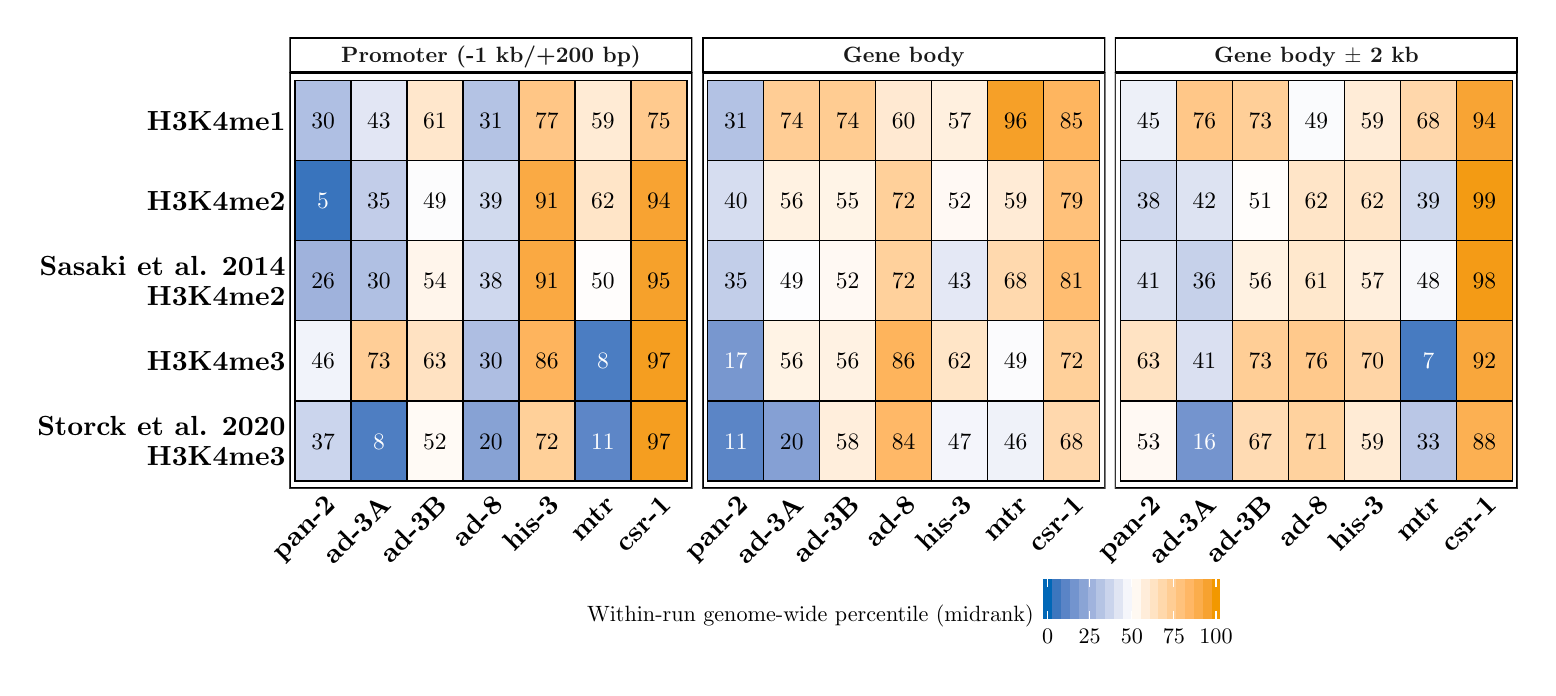
\begin{tikzpicture}[x=1pt,y=1pt]
\definecolor{fillColor}{RGB}{255,255,255}
\path[use as bounding box,fill=fillColor,fill opacity=0.00] (0,0) rectangle (542.02,231.26);
\begin{scope}
\path[clip] (  0.00,  0.00) rectangle (542.02,231.26);
\definecolor{drawColor}{RGB}{255,255,255}
\definecolor{fillColor}{RGB}{255,255,255}

\path[draw=drawColor,line width= 0.7pt,line join=round,line cap=round,fill=fillColor] ( -0.00,  0.00) rectangle (542.02,231.26);
\end{scope}
\begin{scope}
\path[clip] ( 94.59, 64.56) rectangle (240.23,215.09);
\definecolor{drawColor}{RGB}{0,0,0}
\definecolor{fillColor}{RGB}{255,255,255}

\path[draw=drawColor,line width= 1.1pt,line join=round,line cap=round,fill=fillColor] ( 94.59, 64.56) rectangle (240.23,215.09);
\definecolor{fillColor}{RGB}{175,191,227}

\path[draw=drawColor,line width= 0.5pt,fill=fillColor] ( 96.61,183.25) rectangle (116.84,212.19);
\definecolor{fillColor}{RGB}{226,230,244}

\path[draw=drawColor,line width= 0.5pt,fill=fillColor] (116.84,183.25) rectangle (137.07,212.19);
\definecolor{fillColor}{RGB}{255,231,204}

\path[draw=drawColor,line width= 0.5pt,fill=fillColor] (137.07,183.25) rectangle (157.30,212.19);
\definecolor{fillColor}{RGB}{180,195,228}

\path[draw=drawColor,line width= 0.5pt,fill=fillColor] (157.30,183.25) rectangle (177.52,212.19);
\definecolor{fillColor}{RGB}{255,198,134}

\path[draw=drawColor,line width= 0.5pt,fill=fillColor] (177.52,183.25) rectangle (197.75,212.19);
\definecolor{fillColor}{RGB}{255,235,213}

\path[draw=drawColor,line width= 0.5pt,fill=fillColor] (197.75,183.25) rectangle (217.98,212.19);
\definecolor{fillColor}{RGB}{255,202,142}

\path[draw=drawColor,line width= 0.5pt,fill=fillColor] (217.98,183.25) rectangle (238.21,212.19);
\definecolor{fillColor}{RGB}{57,116,189}

\path[draw=drawColor,line width= 0.5pt,fill=fillColor] ( 96.61,154.30) rectangle (116.84,183.25);
\definecolor{fillColor}{RGB}{194,205,233}

\path[draw=drawColor,line width= 0.5pt,fill=fillColor] (116.84,154.30) rectangle (137.07,183.25);
\definecolor{fillColor}{RGB}{252,252,253}

\path[draw=drawColor,line width= 0.5pt,fill=fillColor] (137.07,154.30) rectangle (157.30,183.25);
\definecolor{fillColor}{RGB}{209,218,238}

\path[draw=drawColor,line width= 0.5pt,fill=fillColor] (157.30,154.30) rectangle (177.52,183.25);
\definecolor{fillColor}{RGB}{250,170,68}

\path[draw=drawColor,line width= 0.5pt,fill=fillColor] (177.52,154.30) rectangle (197.75,183.25);
\definecolor{fillColor}{RGB}{255,229,200}

\path[draw=drawColor,line width= 0.5pt,fill=fillColor] (197.75,154.30) rectangle (217.98,183.25);
\definecolor{fillColor}{RGB}{248,163,50}

\path[draw=drawColor,line width= 0.5pt,fill=fillColor] (217.98,154.30) rectangle (238.21,183.25);
\definecolor{fillColor}{RGB}{159,178,220}

\path[draw=drawColor,line width= 0.5pt,fill=fillColor] ( 96.61,125.35) rectangle (116.84,154.30);
\definecolor{fillColor}{RGB}{176,192,227}

\path[draw=drawColor,line width= 0.5pt,fill=fillColor] (116.84,125.35) rectangle (137.07,154.30);
\definecolor{fillColor}{RGB}{255,245,235}

\path[draw=drawColor,line width= 0.5pt,fill=fillColor] (137.07,125.35) rectangle (157.30,154.30);
\definecolor{fillColor}{RGB}{207,216,238}

\path[draw=drawColor,line width= 0.5pt,fill=fillColor] (157.30,125.35) rectangle (177.52,154.30);
\definecolor{fillColor}{RGB}{250,169,66}

\path[draw=drawColor,line width= 0.5pt,fill=fillColor] (177.52,125.35) rectangle (197.75,154.30);
\definecolor{fillColor}{RGB}{255,253,252}

\path[draw=drawColor,line width= 0.5pt,fill=fillColor] (197.75,125.35) rectangle (217.98,154.30);
\definecolor{fillColor}{RGB}{246,161,43}

\path[draw=drawColor,line width= 0.5pt,fill=fillColor] (217.98,125.35) rectangle (238.21,154.30);
\definecolor{fillColor}{RGB}{241,243,250}

\path[draw=drawColor,line width= 0.5pt,fill=fillColor] ( 96.61, 96.40) rectangle (116.84,125.35);
\definecolor{fillColor}{RGB}{255,206,151}

\path[draw=drawColor,line width= 0.5pt,fill=fillColor] (116.84, 96.40) rectangle (137.07,125.35);
\definecolor{fillColor}{RGB}{255,226,194}

\path[draw=drawColor,line width= 0.5pt,fill=fillColor] (137.07, 96.40) rectangle (157.30,125.35);
\definecolor{fillColor}{RGB}{174,190,226}

\path[draw=drawColor,line width= 0.5pt,fill=fillColor] (157.30, 96.40) rectangle (177.52,125.35);
\definecolor{fillColor}{RGB}{254,180,93}

\path[draw=drawColor,line width= 0.5pt,fill=fillColor] (177.52, 96.40) rectangle (197.75,125.35);
\definecolor{fillColor}{RGB}{75,125,194}

\path[draw=drawColor,line width= 0.5pt,fill=fillColor] (197.75, 96.40) rectangle (217.98,125.35);
\definecolor{fillColor}{RGB}{245,158,32}

\path[draw=drawColor,line width= 0.5pt,fill=fillColor] (217.98, 96.40) rectangle (238.21,125.35);
\definecolor{fillColor}{RGB}{203,213,237}

\path[draw=drawColor,line width= 0.5pt,fill=fillColor] ( 96.61, 67.46) rectangle (116.84, 96.40);
\definecolor{fillColor}{RGB}{78,126,194}

\path[draw=drawColor,line width= 0.5pt,fill=fillColor] (116.84, 67.46) rectangle (137.07, 96.40);
\definecolor{fillColor}{RGB}{255,250,245}

\path[draw=drawColor,line width= 0.5pt,fill=fillColor] (137.07, 67.46) rectangle (157.30, 96.40);
\definecolor{fillColor}{RGB}{135,162,212}

\path[draw=drawColor,line width= 0.5pt,fill=fillColor] (157.30, 67.46) rectangle (177.52, 96.40);
\definecolor{fillColor}{RGB}{255,208,153}

\path[draw=drawColor,line width= 0.5pt,fill=fillColor] (177.52, 67.46) rectangle (197.75, 96.40);
\definecolor{fillColor}{RGB}{93,134,199}

\path[draw=drawColor,line width= 0.5pt,fill=fillColor] (197.75, 67.46) rectangle (217.98, 96.40);
\definecolor{fillColor}{RGB}{245,158,32}

\path[draw=drawColor,line width= 0.5pt,fill=fillColor] (217.98, 67.46) rectangle (238.21, 96.40);

\node[text=drawColor,anchor=base,inner sep=0pt, outer sep=0pt, scale=  0.85] at (106.72,194.78) {30};

\node[text=drawColor,anchor=base,inner sep=0pt, outer sep=0pt, scale=  0.85] at (126.95,194.78) {43};

\node[text=drawColor,anchor=base,inner sep=0pt, outer sep=0pt, scale=  0.85] at (147.18,194.78) {61};

\node[text=drawColor,anchor=base,inner sep=0pt, outer sep=0pt, scale=  0.85] at (167.41,194.78) {31};

\node[text=drawColor,anchor=base,inner sep=0pt, outer sep=0pt, scale=  0.85] at (187.64,194.78) {77};

\node[text=drawColor,anchor=base,inner sep=0pt, outer sep=0pt, scale=  0.85] at (207.87,194.78) {59};

\node[text=drawColor,anchor=base,inner sep=0pt, outer sep=0pt, scale=  0.85] at (228.10,194.78) {75};
\definecolor{drawColor}{RGB}{255,255,255}

\node[text=drawColor,anchor=base,inner sep=0pt, outer sep=0pt, scale=  0.85] at (106.72,165.83) {5};
\definecolor{drawColor}{RGB}{0,0,0}

\node[text=drawColor,anchor=base,inner sep=0pt, outer sep=0pt, scale=  0.85] at (126.95,165.83) {35};

\node[text=drawColor,anchor=base,inner sep=0pt, outer sep=0pt, scale=  0.85] at (147.18,165.83) {49};

\node[text=drawColor,anchor=base,inner sep=0pt, outer sep=0pt, scale=  0.85] at (167.41,165.83) {39};

\node[text=drawColor,anchor=base,inner sep=0pt, outer sep=0pt, scale=  0.85] at (187.64,165.83) {91};

\node[text=drawColor,anchor=base,inner sep=0pt, outer sep=0pt, scale=  0.85] at (207.87,165.83) {62};

\node[text=drawColor,anchor=base,inner sep=0pt, outer sep=0pt, scale=  0.85] at (228.10,165.83) {94};

\node[text=drawColor,anchor=base,inner sep=0pt, outer sep=0pt, scale=  0.85] at (106.72,136.89) {26};

\node[text=drawColor,anchor=base,inner sep=0pt, outer sep=0pt, scale=  0.85] at (126.95,136.89) {30};

\node[text=drawColor,anchor=base,inner sep=0pt, outer sep=0pt, scale=  0.85] at (147.18,136.89) {54};

\node[text=drawColor,anchor=base,inner sep=0pt, outer sep=0pt, scale=  0.85] at (167.41,136.89) {38};

\node[text=drawColor,anchor=base,inner sep=0pt, outer sep=0pt, scale=  0.85] at (187.64,136.89) {91};

\node[text=drawColor,anchor=base,inner sep=0pt, outer sep=0pt, scale=  0.85] at (207.87,136.89) {50};

\node[text=drawColor,anchor=base,inner sep=0pt, outer sep=0pt, scale=  0.85] at (228.10,136.89) {95};

\node[text=drawColor,anchor=base,inner sep=0pt, outer sep=0pt, scale=  0.85] at (106.72,107.94) {46};

\node[text=drawColor,anchor=base,inner sep=0pt, outer sep=0pt, scale=  0.85] at (126.95,107.94) {73};

\node[text=drawColor,anchor=base,inner sep=0pt, outer sep=0pt, scale=  0.85] at (147.18,107.94) {63};

\node[text=drawColor,anchor=base,inner sep=0pt, outer sep=0pt, scale=  0.85] at (167.41,107.94) {30};

\node[text=drawColor,anchor=base,inner sep=0pt, outer sep=0pt, scale=  0.85] at (187.64,107.94) {86};
\definecolor{drawColor}{RGB}{255,255,255}

\node[text=drawColor,anchor=base,inner sep=0pt, outer sep=0pt, scale=  0.85] at (207.87,107.94) {8};
\definecolor{drawColor}{RGB}{0,0,0}

\node[text=drawColor,anchor=base,inner sep=0pt, outer sep=0pt, scale=  0.85] at (228.10,107.94) {97};

\node[text=drawColor,anchor=base,inner sep=0pt, outer sep=0pt, scale=  0.85] at (106.72, 78.99) {37};
\definecolor{drawColor}{RGB}{255,255,255}

\node[text=drawColor,anchor=base,inner sep=0pt, outer sep=0pt, scale=  0.85] at (126.95, 78.99) {8};
\definecolor{drawColor}{RGB}{0,0,0}

\node[text=drawColor,anchor=base,inner sep=0pt, outer sep=0pt, scale=  0.85] at (147.18, 78.99) {52};

\node[text=drawColor,anchor=base,inner sep=0pt, outer sep=0pt, scale=  0.85] at (167.41, 78.99) {20};

\node[text=drawColor,anchor=base,inner sep=0pt, outer sep=0pt, scale=  0.85] at (187.64, 78.99) {72};
\definecolor{drawColor}{RGB}{255,255,255}

\node[text=drawColor,anchor=base,inner sep=0pt, outer sep=0pt, scale=  0.85] at (207.87, 78.99) {11};
\definecolor{drawColor}{RGB}{0,0,0}

\node[text=drawColor,anchor=base,inner sep=0pt, outer sep=0pt, scale=  0.85] at (228.10, 78.99) {97};
\definecolor{drawColor}{gray}{0.20}

\path[draw=drawColor,line width= 0.7pt,line join=round,line cap=round] ( 94.59, 64.56) rectangle (240.23,215.09);
\end{scope}
\begin{scope}
\path[clip] (243.73, 64.56) rectangle (389.38,215.09);
\definecolor{drawColor}{RGB}{0,0,0}
\definecolor{fillColor}{RGB}{255,255,255}

\path[draw=drawColor,line width= 1.1pt,line join=round,line cap=round,fill=fillColor] (243.73, 64.56) rectangle (389.38,215.09);
\definecolor{fillColor}{RGB}{179,194,228}

\path[draw=drawColor,line width= 0.5pt,fill=fillColor] (245.76,183.25) rectangle (265.98,212.19);
\definecolor{fillColor}{RGB}{255,205,149}

\path[draw=drawColor,line width= 0.5pt,fill=fillColor] (265.98,183.25) rectangle (286.21,212.19);
\definecolor{fillColor}{RGB}{255,204,146}

\path[draw=drawColor,line width= 0.5pt,fill=fillColor] (286.21,183.25) rectangle (306.44,212.19);
\definecolor{fillColor}{RGB}{255,233,210}

\path[draw=drawColor,line width= 0.5pt,fill=fillColor] (306.44,183.25) rectangle (326.67,212.19);
\definecolor{fillColor}{RGB}{255,240,223}

\path[draw=drawColor,line width= 0.5pt,fill=fillColor] (326.67,183.25) rectangle (346.90,212.19);
\definecolor{fillColor}{RGB}{246,160,40}

\path[draw=drawColor,line width= 0.5pt,fill=fillColor] (346.90,183.25) rectangle (367.13,212.19);
\definecolor{fillColor}{RGB}{254,181,95}

\path[draw=drawColor,line width= 0.5pt,fill=fillColor] (367.13,183.25) rectangle (387.36,212.19);
\definecolor{fillColor}{RGB}{214,221,240}

\path[draw=drawColor,line width= 0.5pt,fill=fillColor] (245.76,154.30) rectangle (265.98,183.25);
\definecolor{fillColor}{RGB}{255,242,226}

\path[draw=drawColor,line width= 0.5pt,fill=fillColor] (265.98,154.30) rectangle (286.21,183.25);
\definecolor{fillColor}{RGB}{255,244,231}

\path[draw=drawColor,line width= 0.5pt,fill=fillColor] (286.21,154.30) rectangle (306.44,183.25);
\definecolor{fillColor}{RGB}{255,208,154}

\path[draw=drawColor,line width= 0.5pt,fill=fillColor] (306.44,154.30) rectangle (326.67,183.25);
\definecolor{fillColor}{RGB}{255,249,244}

\path[draw=drawColor,line width= 0.5pt,fill=fillColor] (326.67,154.30) rectangle (346.90,183.25);
\definecolor{fillColor}{RGB}{255,235,214}

\path[draw=drawColor,line width= 0.5pt,fill=fillColor] (346.90,154.30) rectangle (367.13,183.25);
\definecolor{fillColor}{RGB}{255,193,122}

\path[draw=drawColor,line width= 0.5pt,fill=fillColor] (367.13,154.30) rectangle (387.36,183.25);
\definecolor{fillColor}{RGB}{194,206,233}

\path[draw=drawColor,line width= 0.5pt,fill=fillColor] (245.76,125.35) rectangle (265.98,154.30);
\definecolor{fillColor}{RGB}{253,253,254}

\path[draw=drawColor,line width= 0.5pt,fill=fillColor] (265.98,125.35) rectangle (286.21,154.30);
\definecolor{fillColor}{RGB}{255,249,243}

\path[draw=drawColor,line width= 0.5pt,fill=fillColor] (286.21,125.35) rectangle (306.44,154.30);
\definecolor{fillColor}{RGB}{255,209,156}

\path[draw=drawColor,line width= 0.5pt,fill=fillColor] (306.44,125.35) rectangle (326.67,154.30);
\definecolor{fillColor}{RGB}{228,232,245}

\path[draw=drawColor,line width= 0.5pt,fill=fillColor] (326.67,125.35) rectangle (346.90,154.30);
\definecolor{fillColor}{RGB}{255,217,174}

\path[draw=drawColor,line width= 0.5pt,fill=fillColor] (346.90,125.35) rectangle (367.13,154.30);
\definecolor{fillColor}{RGB}{255,189,113}

\path[draw=drawColor,line width= 0.5pt,fill=fillColor] (367.13,125.35) rectangle (387.36,154.30);
\definecolor{fillColor}{RGB}{120,151,207}

\path[draw=drawColor,line width= 0.5pt,fill=fillColor] (245.76, 96.40) rectangle (265.98,125.35);
\definecolor{fillColor}{RGB}{255,243,229}

\path[draw=drawColor,line width= 0.5pt,fill=fillColor] (265.98, 96.40) rectangle (286.21,125.35);
\definecolor{fillColor}{RGB}{255,242,227}

\path[draw=drawColor,line width= 0.5pt,fill=fillColor] (286.21, 96.40) rectangle (306.44,125.35);
\definecolor{fillColor}{RGB}{254,180,92}

\path[draw=drawColor,line width= 0.5pt,fill=fillColor] (306.44, 96.40) rectangle (326.67,125.35);
\definecolor{fillColor}{RGB}{255,229,199}

\path[draw=drawColor,line width= 0.5pt,fill=fillColor] (326.67, 96.40) rectangle (346.90,125.35);
\definecolor{fillColor}{RGB}{251,251,253}

\path[draw=drawColor,line width= 0.5pt,fill=fillColor] (346.90, 96.40) rectangle (367.13,125.35);
\definecolor{fillColor}{RGB}{255,208,154}

\path[draw=drawColor,line width= 0.5pt,fill=fillColor] (367.13, 96.40) rectangle (387.36,125.35);
\definecolor{fillColor}{RGB}{91,133,198}

\path[draw=drawColor,line width= 0.5pt,fill=fillColor] (245.76, 67.46) rectangle (265.98, 96.40);
\definecolor{fillColor}{RGB}{133,160,212}

\path[draw=drawColor,line width= 0.5pt,fill=fillColor] (265.98, 67.46) rectangle (286.21, 96.40);
\definecolor{fillColor}{RGB}{255,238,220}

\path[draw=drawColor,line width= 0.5pt,fill=fillColor] (286.21, 67.46) rectangle (306.44, 96.40);
\definecolor{fillColor}{RGB}{255,184,103}

\path[draw=drawColor,line width= 0.5pt,fill=fillColor] (306.44, 67.46) rectangle (326.67, 96.40);
\definecolor{fillColor}{RGB}{244,245,251}

\path[draw=drawColor,line width= 0.5pt,fill=fillColor] (326.67, 67.46) rectangle (346.90, 96.40);
\definecolor{fillColor}{RGB}{239,242,249}

\path[draw=drawColor,line width= 0.5pt,fill=fillColor] (346.90, 67.46) rectangle (367.13, 96.40);
\definecolor{fillColor}{RGB}{255,216,173}

\path[draw=drawColor,line width= 0.5pt,fill=fillColor] (367.13, 67.46) rectangle (387.36, 96.40);

\node[text=drawColor,anchor=base,inner sep=0pt, outer sep=0pt, scale=  0.85] at (255.87,194.78) {31};

\node[text=drawColor,anchor=base,inner sep=0pt, outer sep=0pt, scale=  0.85] at (276.10,194.78) {74};

\node[text=drawColor,anchor=base,inner sep=0pt, outer sep=0pt, scale=  0.85] at (296.33,194.78) {74};

\node[text=drawColor,anchor=base,inner sep=0pt, outer sep=0pt, scale=  0.85] at (316.56,194.78) {60};

\node[text=drawColor,anchor=base,inner sep=0pt, outer sep=0pt, scale=  0.85] at (336.78,194.78) {57};

\node[text=drawColor,anchor=base,inner sep=0pt, outer sep=0pt, scale=  0.85] at (357.01,194.78) {96};

\node[text=drawColor,anchor=base,inner sep=0pt, outer sep=0pt, scale=  0.85] at (377.24,194.78) {85};

\node[text=drawColor,anchor=base,inner sep=0pt, outer sep=0pt, scale=  0.85] at (255.87,165.83) {40};

\node[text=drawColor,anchor=base,inner sep=0pt, outer sep=0pt, scale=  0.85] at (276.10,165.83) {56};

\node[text=drawColor,anchor=base,inner sep=0pt, outer sep=0pt, scale=  0.85] at (296.33,165.83) {55};

\node[text=drawColor,anchor=base,inner sep=0pt, outer sep=0pt, scale=  0.85] at (316.56,165.83) {72};

\node[text=drawColor,anchor=base,inner sep=0pt, outer sep=0pt, scale=  0.85] at (336.78,165.83) {52};

\node[text=drawColor,anchor=base,inner sep=0pt, outer sep=0pt, scale=  0.85] at (357.01,165.83) {59};

\node[text=drawColor,anchor=base,inner sep=0pt, outer sep=0pt, scale=  0.85] at (377.24,165.83) {79};

\node[text=drawColor,anchor=base,inner sep=0pt, outer sep=0pt, scale=  0.85] at (255.87,136.89) {35};

\node[text=drawColor,anchor=base,inner sep=0pt, outer sep=0pt, scale=  0.85] at (276.10,136.89) {49};

\node[text=drawColor,anchor=base,inner sep=0pt, outer sep=0pt, scale=  0.85] at (296.33,136.89) {52};

\node[text=drawColor,anchor=base,inner sep=0pt, outer sep=0pt, scale=  0.85] at (316.56,136.89) {72};

\node[text=drawColor,anchor=base,inner sep=0pt, outer sep=0pt, scale=  0.85] at (336.78,136.89) {43};

\node[text=drawColor,anchor=base,inner sep=0pt, outer sep=0pt, scale=  0.85] at (357.01,136.89) {68};

\node[text=drawColor,anchor=base,inner sep=0pt, outer sep=0pt, scale=  0.85] at (377.24,136.89) {81};
\definecolor{drawColor}{RGB}{255,255,255}

\node[text=drawColor,anchor=base,inner sep=0pt, outer sep=0pt, scale=  0.85] at (255.87,107.94) {17};
\definecolor{drawColor}{RGB}{0,0,0}

\node[text=drawColor,anchor=base,inner sep=0pt, outer sep=0pt, scale=  0.85] at (276.10,107.94) {56};

\node[text=drawColor,anchor=base,inner sep=0pt, outer sep=0pt, scale=  0.85] at (296.33,107.94) {56};

\node[text=drawColor,anchor=base,inner sep=0pt, outer sep=0pt, scale=  0.85] at (316.56,107.94) {86};

\node[text=drawColor,anchor=base,inner sep=0pt, outer sep=0pt, scale=  0.85] at (336.78,107.94) {62};

\node[text=drawColor,anchor=base,inner sep=0pt, outer sep=0pt, scale=  0.85] at (357.01,107.94) {49};

\node[text=drawColor,anchor=base,inner sep=0pt, outer sep=0pt, scale=  0.85] at (377.24,107.94) {72};
\definecolor{drawColor}{RGB}{255,255,255}

\node[text=drawColor,anchor=base,inner sep=0pt, outer sep=0pt, scale=  0.85] at (255.87, 78.99) {11};
\definecolor{drawColor}{RGB}{0,0,0}

\node[text=drawColor,anchor=base,inner sep=0pt, outer sep=0pt, scale=  0.85] at (276.10, 78.99) {20};

\node[text=drawColor,anchor=base,inner sep=0pt, outer sep=0pt, scale=  0.85] at (296.33, 78.99) {58};

\node[text=drawColor,anchor=base,inner sep=0pt, outer sep=0pt, scale=  0.85] at (316.56, 78.99) {84};

\node[text=drawColor,anchor=base,inner sep=0pt, outer sep=0pt, scale=  0.85] at (336.78, 78.99) {47};

\node[text=drawColor,anchor=base,inner sep=0pt, outer sep=0pt, scale=  0.85] at (357.01, 78.99) {46};

\node[text=drawColor,anchor=base,inner sep=0pt, outer sep=0pt, scale=  0.85] at (377.24, 78.99) {68};
\definecolor{drawColor}{gray}{0.20}

\path[draw=drawColor,line width= 0.7pt,line join=round,line cap=round] (243.73, 64.56) rectangle (389.38,215.09);
\end{scope}
\begin{scope}
\path[clip] (392.88, 64.56) rectangle (538.52,215.09);
\definecolor{drawColor}{RGB}{0,0,0}
\definecolor{fillColor}{RGB}{255,255,255}

\path[draw=drawColor,line width= 1.1pt,line join=round,line cap=round,fill=fillColor] (392.88, 64.56) rectangle (538.52,215.09);
\definecolor{fillColor}{RGB}{237,240,248}

\path[draw=drawColor,line width= 0.5pt,fill=fillColor] (394.90,183.25) rectangle (415.13,212.19);
\definecolor{fillColor}{RGB}{255,199,136}

\path[draw=drawColor,line width= 0.5pt,fill=fillColor] (415.13,183.25) rectangle (435.36,212.19);
\definecolor{fillColor}{RGB}{255,207,152}

\path[draw=drawColor,line width= 0.5pt,fill=fillColor] (435.36,183.25) rectangle (455.59,212.19);
\definecolor{fillColor}{RGB}{250,251,253}

\path[draw=drawColor,line width= 0.5pt,fill=fillColor] (455.59,183.25) rectangle (475.82,212.19);
\definecolor{fillColor}{RGB}{255,236,215}

\path[draw=drawColor,line width= 0.5pt,fill=fillColor] (475.82,183.25) rectangle (496.04,212.19);
\definecolor{fillColor}{RGB}{255,215,171}

\path[draw=drawColor,line width= 0.5pt,fill=fillColor] (496.04,183.25) rectangle (516.27,212.19);
\definecolor{fillColor}{RGB}{248,164,52}

\path[draw=drawColor,line width= 0.5pt,fill=fillColor] (516.27,183.25) rectangle (536.50,212.19);
\definecolor{fillColor}{RGB}{208,217,238}

\path[draw=drawColor,line width= 0.5pt,fill=fillColor] (394.90,154.30) rectangle (415.13,183.25);
\definecolor{fillColor}{RGB}{221,227,242}

\path[draw=drawColor,line width= 0.5pt,fill=fillColor] (415.13,154.30) rectangle (435.36,183.25);
\definecolor{fillColor}{RGB}{255,253,251}

\path[draw=drawColor,line width= 0.5pt,fill=fillColor] (435.36,154.30) rectangle (455.59,183.25);
\definecolor{fillColor}{RGB}{255,229,200}

\path[draw=drawColor,line width= 0.5pt,fill=fillColor] (455.59,154.30) rectangle (475.82,183.25);

\path[draw=drawColor,line width= 0.5pt,fill=fillColor] (475.82,154.30) rectangle (496.04,183.25);
\definecolor{fillColor}{RGB}{209,218,238}

\path[draw=drawColor,line width= 0.5pt,fill=fillColor] (496.04,154.30) rectangle (516.27,183.25);
\definecolor{fillColor}{RGB}{243,155,19}

\path[draw=drawColor,line width= 0.5pt,fill=fillColor] (516.27,154.30) rectangle (536.50,183.25);
\definecolor{fillColor}{RGB}{219,225,241}

\path[draw=drawColor,line width= 0.5pt,fill=fillColor] (394.90,125.35) rectangle (415.13,154.30);
\definecolor{fillColor}{RGB}{198,209,234}

\path[draw=drawColor,line width= 0.5pt,fill=fillColor] (415.13,125.35) rectangle (435.36,154.30);
\definecolor{fillColor}{RGB}{255,242,226}

\path[draw=drawColor,line width= 0.5pt,fill=fillColor] (435.36,125.35) rectangle (455.59,154.30);
\definecolor{fillColor}{RGB}{255,232,205}

\path[draw=drawColor,line width= 0.5pt,fill=fillColor] (455.59,125.35) rectangle (475.82,154.30);
\definecolor{fillColor}{RGB}{255,239,221}

\path[draw=drawColor,line width= 0.5pt,fill=fillColor] (475.82,125.35) rectangle (496.04,154.30);
\definecolor{fillColor}{RGB}{248,249,252}

\path[draw=drawColor,line width= 0.5pt,fill=fillColor] (496.04,125.35) rectangle (516.27,154.30);
\definecolor{fillColor}{RGB}{244,155,22}

\path[draw=drawColor,line width= 0.5pt,fill=fillColor] (516.27,125.35) rectangle (536.50,154.30);
\definecolor{fillColor}{RGB}{255,227,195}

\path[draw=drawColor,line width= 0.5pt,fill=fillColor] (394.90, 96.40) rectangle (415.13,125.35);
\definecolor{fillColor}{RGB}{218,224,241}

\path[draw=drawColor,line width= 0.5pt,fill=fillColor] (415.13, 96.40) rectangle (435.36,125.35);
\definecolor{fillColor}{RGB}{255,206,150}

\path[draw=drawColor,line width= 0.5pt,fill=fillColor] (435.36, 96.40) rectangle (455.59,125.35);
\definecolor{fillColor}{RGB}{255,201,140}

\path[draw=drawColor,line width= 0.5pt,fill=fillColor] (455.59, 96.40) rectangle (475.82,125.35);
\definecolor{fillColor}{RGB}{255,213,166}

\path[draw=drawColor,line width= 0.5pt,fill=fillColor] (475.82, 96.40) rectangle (496.04,125.35);
\definecolor{fillColor}{RGB}{71,123,193}

\path[draw=drawColor,line width= 0.5pt,fill=fillColor] (496.04, 96.40) rectangle (516.27,125.35);
\definecolor{fillColor}{RGB}{249,167,60}

\path[draw=drawColor,line width= 0.5pt,fill=fillColor] (516.27, 96.40) rectangle (536.50,125.35);
\definecolor{fillColor}{RGB}{255,249,243}

\path[draw=drawColor,line width= 0.5pt,fill=fillColor] (394.90, 67.46) rectangle (415.13, 96.40);
\definecolor{fillColor}{RGB}{116,148,206}

\path[draw=drawColor,line width= 0.5pt,fill=fillColor] (415.13, 67.46) rectangle (435.36, 96.40);
\definecolor{fillColor}{RGB}{255,219,179}

\path[draw=drawColor,line width= 0.5pt,fill=fillColor] (435.36, 67.46) rectangle (455.59, 96.40);
\definecolor{fillColor}{RGB}{255,210,158}

\path[draw=drawColor,line width= 0.5pt,fill=fillColor] (455.59, 67.46) rectangle (475.82, 96.40);
\definecolor{fillColor}{RGB}{255,235,213}

\path[draw=drawColor,line width= 0.5pt,fill=fillColor] (475.82, 67.46) rectangle (496.04, 96.40);
\definecolor{fillColor}{RGB}{186,199,230}

\path[draw=drawColor,line width= 0.5pt,fill=fillColor] (496.04, 67.46) rectangle (516.27, 96.40);
\definecolor{fillColor}{RGB}{252,176,82}

\path[draw=drawColor,line width= 0.5pt,fill=fillColor] (516.27, 67.46) rectangle (536.50, 96.40);

\node[text=drawColor,anchor=base,inner sep=0pt, outer sep=0pt, scale=  0.85] at (405.02,194.78) {45};

\node[text=drawColor,anchor=base,inner sep=0pt, outer sep=0pt, scale=  0.85] at (425.24,194.78) {76};

\node[text=drawColor,anchor=base,inner sep=0pt, outer sep=0pt, scale=  0.85] at (445.47,194.78) {73};

\node[text=drawColor,anchor=base,inner sep=0pt, outer sep=0pt, scale=  0.85] at (465.70,194.78) {49};

\node[text=drawColor,anchor=base,inner sep=0pt, outer sep=0pt, scale=  0.85] at (485.93,194.78) {59};

\node[text=drawColor,anchor=base,inner sep=0pt, outer sep=0pt, scale=  0.85] at (506.16,194.78) {68};

\node[text=drawColor,anchor=base,inner sep=0pt, outer sep=0pt, scale=  0.85] at (526.39,194.78) {94};

\node[text=drawColor,anchor=base,inner sep=0pt, outer sep=0pt, scale=  0.85] at (405.02,165.83) {38};

\node[text=drawColor,anchor=base,inner sep=0pt, outer sep=0pt, scale=  0.85] at (425.24,165.83) {42};

\node[text=drawColor,anchor=base,inner sep=0pt, outer sep=0pt, scale=  0.85] at (445.47,165.83) {51};

\node[text=drawColor,anchor=base,inner sep=0pt, outer sep=0pt, scale=  0.85] at (465.70,165.83) {62};

\node[text=drawColor,anchor=base,inner sep=0pt, outer sep=0pt, scale=  0.85] at (485.93,165.83) {62};

\node[text=drawColor,anchor=base,inner sep=0pt, outer sep=0pt, scale=  0.85] at (506.16,165.83) {39};

\node[text=drawColor,anchor=base,inner sep=0pt, outer sep=0pt, scale=  0.85] at (526.39,165.83) {99};

\node[text=drawColor,anchor=base,inner sep=0pt, outer sep=0pt, scale=  0.85] at (405.02,136.89) {41};

\node[text=drawColor,anchor=base,inner sep=0pt, outer sep=0pt, scale=  0.85] at (425.24,136.89) {36};

\node[text=drawColor,anchor=base,inner sep=0pt, outer sep=0pt, scale=  0.85] at (445.47,136.89) {56};

\node[text=drawColor,anchor=base,inner sep=0pt, outer sep=0pt, scale=  0.85] at (465.70,136.89) {61};

\node[text=drawColor,anchor=base,inner sep=0pt, outer sep=0pt, scale=  0.85] at (485.93,136.89) {57};

\node[text=drawColor,anchor=base,inner sep=0pt, outer sep=0pt, scale=  0.85] at (506.16,136.89) {48};

\node[text=drawColor,anchor=base,inner sep=0pt, outer sep=0pt, scale=  0.85] at (526.39,136.89) {98};

\node[text=drawColor,anchor=base,inner sep=0pt, outer sep=0pt, scale=  0.85] at (405.02,107.94) {63};

\node[text=drawColor,anchor=base,inner sep=0pt, outer sep=0pt, scale=  0.85] at (425.24,107.94) {41};

\node[text=drawColor,anchor=base,inner sep=0pt, outer sep=0pt, scale=  0.85] at (445.47,107.94) {73};

\node[text=drawColor,anchor=base,inner sep=0pt, outer sep=0pt, scale=  0.85] at (465.70,107.94) {76};

\node[text=drawColor,anchor=base,inner sep=0pt, outer sep=0pt, scale=  0.85] at (485.93,107.94) {70};
\definecolor{drawColor}{RGB}{255,255,255}

\node[text=drawColor,anchor=base,inner sep=0pt, outer sep=0pt, scale=  0.85] at (506.16,107.94) {7};
\definecolor{drawColor}{RGB}{0,0,0}

\node[text=drawColor,anchor=base,inner sep=0pt, outer sep=0pt, scale=  0.85] at (526.39,107.94) {92};

\node[text=drawColor,anchor=base,inner sep=0pt, outer sep=0pt, scale=  0.85] at (405.02, 78.99) {53};
\definecolor{drawColor}{RGB}{255,255,255}

\node[text=drawColor,anchor=base,inner sep=0pt, outer sep=0pt, scale=  0.85] at (425.24, 78.99) {16};
\definecolor{drawColor}{RGB}{0,0,0}

\node[text=drawColor,anchor=base,inner sep=0pt, outer sep=0pt, scale=  0.85] at (445.47, 78.99) {67};

\node[text=drawColor,anchor=base,inner sep=0pt, outer sep=0pt, scale=  0.85] at (465.70, 78.99) {71};

\node[text=drawColor,anchor=base,inner sep=0pt, outer sep=0pt, scale=  0.85] at (485.93, 78.99) {59};

\node[text=drawColor,anchor=base,inner sep=0pt, outer sep=0pt, scale=  0.85] at (506.16, 78.99) {33};

\node[text=drawColor,anchor=base,inner sep=0pt, outer sep=0pt, scale=  0.85] at (526.39, 78.99) {88};
\definecolor{drawColor}{gray}{0.20}

\path[draw=drawColor,line width= 0.7pt,line join=round,line cap=round] (392.88, 64.56) rectangle (538.52,215.09);
\end{scope}
\begin{scope}
\path[clip] ( 94.59,215.09) rectangle (240.23,227.76);
\definecolor{drawColor}{RGB}{0,0,0}
\definecolor{fillColor}{RGB}{255,255,255}

\path[draw=drawColor,line width= 1.1pt,line join=round,line cap=round,fill=fillColor] ( 94.59,215.09) rectangle (240.23,227.76);
\definecolor{drawColor}{gray}{0.10}

\node[text=drawColor,anchor=base,inner sep=0pt, outer sep=0pt, scale=  0.80] at (167.41,218.67) {\bfseries Promoter (-1 kb/+200 bp)};
\end{scope}
\begin{scope}
\path[clip] (243.73,215.09) rectangle (389.38,227.76);
\definecolor{drawColor}{RGB}{0,0,0}
\definecolor{fillColor}{RGB}{255,255,255}

\path[draw=drawColor,line width= 1.1pt,line join=round,line cap=round,fill=fillColor] (243.73,215.09) rectangle (389.38,227.76);
\definecolor{drawColor}{gray}{0.10}

\node[text=drawColor,anchor=base,inner sep=0pt, outer sep=0pt, scale=  0.80] at (316.56,218.67) {\bfseries Gene body};
\end{scope}
\begin{scope}
\path[clip] (392.88,215.09) rectangle (538.52,227.76);
\definecolor{drawColor}{RGB}{0,0,0}
\definecolor{fillColor}{RGB}{255,255,255}

\path[draw=drawColor,line width= 1.1pt,line join=round,line cap=round,fill=fillColor] (392.88,215.09) rectangle (538.52,227.76);
\definecolor{drawColor}{gray}{0.10}

\node[text=drawColor,anchor=base,inner sep=0pt, outer sep=0pt, scale=  0.80] at (465.70,218.67) {\bfseries Gene body $\pm$ 2 kb};
\end{scope}
\begin{scope}
\path[clip] (  0.00,  0.00) rectangle (542.02,231.26);
\definecolor{drawColor}{RGB}{0,0,0}

\node[text=drawColor,rotate= 45.00,anchor=base east,inner sep=0pt, outer sep=0pt, scale=  1.00] at (111.60, 58.28) {\bfseries pan-2};

\node[text=drawColor,rotate= 45.00,anchor=base east,inner sep=0pt, outer sep=0pt, scale=  1.00] at (131.83, 58.28) {\bfseries ad-3A};

\node[text=drawColor,rotate= 45.00,anchor=base east,inner sep=0pt, outer sep=0pt, scale=  1.00] at (152.06, 58.28) {\bfseries ad-3B};

\node[text=drawColor,rotate= 45.00,anchor=base east,inner sep=0pt, outer sep=0pt, scale=  1.00] at (172.29, 58.28) {\bfseries ad-8};

\node[text=drawColor,rotate= 45.00,anchor=base east,inner sep=0pt, outer sep=0pt, scale=  1.00] at (192.52, 58.28) {\bfseries his-3};

\node[text=drawColor,rotate= 45.00,anchor=base east,inner sep=0pt, outer sep=0pt, scale=  1.00] at (212.75, 58.28) {\bfseries mtr};

\node[text=drawColor,rotate= 45.00,anchor=base east,inner sep=0pt, outer sep=0pt, scale=  1.00] at (232.98, 58.28) {\bfseries csr-1};
\end{scope}
\begin{scope}
\path[clip] (  0.00,  0.00) rectangle (542.02,231.26);
\definecolor{drawColor}{RGB}{0,0,0}

\node[text=drawColor,rotate= 45.00,anchor=base east,inner sep=0pt, outer sep=0pt, scale=  1.00] at (260.75, 58.28) {\bfseries pan-2};

\node[text=drawColor,rotate= 45.00,anchor=base east,inner sep=0pt, outer sep=0pt, scale=  1.00] at (280.98, 58.28) {\bfseries ad-3A};

\node[text=drawColor,rotate= 45.00,anchor=base east,inner sep=0pt, outer sep=0pt, scale=  1.00] at (301.21, 58.28) {\bfseries ad-3B};

\node[text=drawColor,rotate= 45.00,anchor=base east,inner sep=0pt, outer sep=0pt, scale=  1.00] at (321.44, 58.28) {\bfseries ad-8};

\node[text=drawColor,rotate= 45.00,anchor=base east,inner sep=0pt, outer sep=0pt, scale=  1.00] at (341.66, 58.28) {\bfseries his-3};

\node[text=drawColor,rotate= 45.00,anchor=base east,inner sep=0pt, outer sep=0pt, scale=  1.00] at (361.89, 58.28) {\bfseries mtr};

\node[text=drawColor,rotate= 45.00,anchor=base east,inner sep=0pt, outer sep=0pt, scale=  1.00] at (382.12, 58.28) {\bfseries csr-1};
\end{scope}
\begin{scope}
\path[clip] (  0.00,  0.00) rectangle (542.02,231.26);
\definecolor{drawColor}{RGB}{0,0,0}

\node[text=drawColor,rotate= 45.00,anchor=base east,inner sep=0pt, outer sep=0pt, scale=  1.00] at (409.90, 58.28) {\bfseries pan-2};

\node[text=drawColor,rotate= 45.00,anchor=base east,inner sep=0pt, outer sep=0pt, scale=  1.00] at (430.12, 58.28) {\bfseries ad-3A};

\node[text=drawColor,rotate= 45.00,anchor=base east,inner sep=0pt, outer sep=0pt, scale=  1.00] at (450.35, 58.28) {\bfseries ad-3B};

\node[text=drawColor,rotate= 45.00,anchor=base east,inner sep=0pt, outer sep=0pt, scale=  1.00] at (470.58, 58.28) {\bfseries ad-8};

\node[text=drawColor,rotate= 45.00,anchor=base east,inner sep=0pt, outer sep=0pt, scale=  1.00] at (490.81, 58.28) {\bfseries his-3};

\node[text=drawColor,rotate= 45.00,anchor=base east,inner sep=0pt, outer sep=0pt, scale=  1.00] at (511.04, 58.28) {\bfseries mtr};

\node[text=drawColor,rotate= 45.00,anchor=base east,inner sep=0pt, outer sep=0pt, scale=  1.00] at (531.27, 58.28) {\bfseries csr-1};
\end{scope}
\begin{scope}
\path[clip] (  0.00,  0.00) rectangle (542.02,231.26);
\definecolor{drawColor}{RGB}{0,0,0}

\node[text=drawColor,anchor=base east,inner sep=0pt, outer sep=0pt, scale=  1.00] at ( 93.19, 83.88) {\bfseries Storck et al. 2020};

\node[text=drawColor,anchor=base east,inner sep=0pt, outer sep=0pt, scale=  1.00] at ( 93.19, 73.08) {\bfseries H3K4me3};

\node[text=drawColor,anchor=base east,inner sep=0pt, outer sep=0pt, scale=  1.00] at ( 93.19,107.43) {\bfseries H3K4me3};

\node[text=drawColor,anchor=base east,inner sep=0pt, outer sep=0pt, scale=  1.00] at ( 93.19,141.77) {\bfseries Sasaki et al. 2014};

\node[text=drawColor,anchor=base east,inner sep=0pt, outer sep=0pt, scale=  1.00] at ( 93.19,130.97) {\bfseries H3K4me2};

\node[text=drawColor,anchor=base east,inner sep=0pt, outer sep=0pt, scale=  1.00] at ( 93.19,165.32) {\bfseries H3K4me2};

\node[text=drawColor,anchor=base east,inner sep=0pt, outer sep=0pt, scale=  1.00] at ( 93.19,194.27) {\bfseries H3K4me1};
\end{scope}
\begin{scope}
\path[clip] (  0.00,  0.00) rectangle (542.02,231.26);
\definecolor{fillColor}{RGB}{255,255,255}

\path[fill=fillColor] (198.62,  3.50) rectangle (434.50, 35.52);
\end{scope}
\begin{scope}
\path[clip] (  0.00,  0.00) rectangle (542.02,231.26);
\definecolor{drawColor}{RGB}{0,0,0}

\node[text=drawColor,anchor=base west,inner sep=0pt, outer sep=0pt, scale=  0.80] at (202.12, 16.75) {Within-run genome-wide percentile (midrank)};
\end{scope}
\begin{scope}
\path[clip] (  0.00,  0.00) rectangle (542.02,231.26);
\definecolor{fillColor}{RGB}{0,103,183}

\path[fill=fillColor] (366.98, 17.56) rectangle (370.18, 32.02);
\definecolor{fillColor}{RGB}{60,118,190}

\path[fill=fillColor] (370.18, 17.56) rectangle (373.38, 32.02);
\definecolor{fillColor}{RGB}{90,132,198}

\path[fill=fillColor] (373.38, 17.56) rectangle (376.58, 32.02);
\definecolor{fillColor}{RGB}{115,148,206}

\path[fill=fillColor] (376.58, 17.56) rectangle (379.78, 32.02);
\definecolor{fillColor}{RGB}{138,164,213}

\path[fill=fillColor] (379.78, 17.56) rectangle (382.98, 32.02);
\definecolor{fillColor}{RGB}{160,179,221}

\path[fill=fillColor] (382.98, 17.56) rectangle (386.18, 32.02);
\definecolor{fillColor}{RGB}{181,196,228}

\path[fill=fillColor] (386.18, 17.56) rectangle (389.38, 32.02);
\definecolor{fillColor}{RGB}{202,212,236}

\path[fill=fillColor] (389.38, 17.56) rectangle (392.58, 32.02);
\definecolor{fillColor}{RGB}{224,229,243}

\path[fill=fillColor] (392.58, 17.56) rectangle (395.79, 32.02);
\definecolor{fillColor}{RGB}{245,246,251}

\path[fill=fillColor] (395.79, 17.56) rectangle (398.99, 32.02);
\definecolor{fillColor}{RGB}{255,249,242}

\path[fill=fillColor] (398.99, 17.56) rectangle (402.19, 32.02);
\definecolor{fillColor}{RGB}{255,237,218}

\path[fill=fillColor] (402.19, 17.56) rectangle (405.39, 32.02);
\definecolor{fillColor}{RGB}{255,227,195}

\path[fill=fillColor] (405.39, 17.56) rectangle (408.59, 32.02);
\definecolor{fillColor}{RGB}{255,216,171}

\path[fill=fillColor] (408.59, 17.56) rectangle (411.79, 32.02);
\definecolor{fillColor}{RGB}{255,205,148}

\path[fill=fillColor] (411.79, 17.56) rectangle (414.99, 32.02);
\definecolor{fillColor}{RGB}{255,194,124}

\path[fill=fillColor] (414.99, 17.56) rectangle (418.19, 32.02);
\definecolor{fillColor}{RGB}{255,183,101}

\path[fill=fillColor] (418.19, 17.56) rectangle (421.39, 32.02);
\definecolor{fillColor}{RGB}{251,173,76}

\path[fill=fillColor] (421.39, 17.56) rectangle (424.59, 32.02);
\definecolor{fillColor}{RGB}{247,162,48}

\path[fill=fillColor] (424.59, 17.56) rectangle (427.79, 32.02);
\definecolor{fillColor}{RGB}{242,152,0}

\path[fill=fillColor] (427.79, 17.56) rectangle (431.00, 32.02);
\end{scope}
\begin{scope}
\path[clip] (  0.00,  0.00) rectangle (542.02,231.26);
\definecolor{drawColor}{RGB}{255,255,255}

\path[draw=drawColor,line width= 0.4pt,line join=round] (368.58, 20.46) --
	(368.58, 17.56);

\path[draw=drawColor,line width= 0.4pt,line join=round] (383.78, 20.46) --
	(383.78, 17.56);

\path[draw=drawColor,line width= 0.4pt,line join=round] (398.99, 20.46) --
	(398.99, 17.56);

\path[draw=drawColor,line width= 0.4pt,line join=round] (414.19, 20.46) --
	(414.19, 17.56);

\path[draw=drawColor,line width= 0.4pt,line join=round] (429.40, 20.46) --
	(429.40, 17.56);

\path[draw=drawColor,line width= 0.4pt,line join=round] (368.58, 29.13) --
	(368.58, 32.02);

\path[draw=drawColor,line width= 0.4pt,line join=round] (383.78, 29.13) --
	(383.78, 32.02);

\path[draw=drawColor,line width= 0.4pt,line join=round] (398.99, 29.13) --
	(398.99, 32.02);

\path[draw=drawColor,line width= 0.4pt,line join=round] (414.19, 29.13) --
	(414.19, 32.02);

\path[draw=drawColor,line width= 0.4pt,line join=round] (429.40, 29.13) --
	(429.40, 32.02);
\end{scope}
\begin{scope}
\path[clip] (  0.00,  0.00) rectangle (542.02,231.26);
\definecolor{drawColor}{RGB}{0,0,0}

\node[text=drawColor,anchor=base,inner sep=0pt, outer sep=0pt, scale=  0.80] at (368.58,  8.56) {0};

\node[text=drawColor,anchor=base,inner sep=0pt, outer sep=0pt, scale=  0.80] at (383.78,  8.56) {25};

\node[text=drawColor,anchor=base,inner sep=0pt, outer sep=0pt, scale=  0.80] at (398.99,  8.56) {50};

\node[text=drawColor,anchor=base,inner sep=0pt, outer sep=0pt, scale=  0.80] at (414.19,  8.56) {75};

\node[text=drawColor,anchor=base,inner sep=0pt, outer sep=0pt, scale=  0.80] at (429.40,  8.56) {100};
\end{scope}
\end{tikzpicture}
